\documentclass{uwstat572}

%%\setlength{\oddsidemargin}{0.25in}
%%\setlength{\textwidth}{6in}
%%\setlength{\topmargin}{0.5in}
%%\setlength{\textheight}{9in}

\renewcommand{\baselinestretch}{1.5} 
\usepackage{bm}
\usepackage{amssymb}
\usepackage{graphicx}
\usepackage{ulem}
\usepackage{color}
\usepackage{amsmath}
\usepackage{makecell}
\allowdisplaybreaks
  %\bibliographystyle{plainnat}		  %\bibliographystyle{plainnat}
  		  

\newcommand{\vmdel}[1]{\sout{#1}}
\newcommand{\vmadd}[1]{\textbf{\color{red}{#1}}}
\newcommand{\vmcomment}[1]{({\color{blue}{VM's comment:}} \textbf{\color{blue}{#1}})}
%\bibliographystyle{plainnat}

\begin{document}
%%\maketitle

\begin{center}
  {\LARGE A technical report on Semi-Markov Models with Phase-Type Sojourn Distributions}\\\ \\
  {Rahul Biswas \\ 
    Department of Statistics, University of Washington Seattle, WA, 98195, USA
  }
\end{center}
\nocite{*}
\section*{The paper}
This report is based on \textit{Semi-Markov Models with Phase-Type Sojourn Distributions} written by Andrew C. Titman and Linda D. Sharples, and published in the Biometrics in 2010 (Titman \& Sharples; 2010).

\section{Introduction}

Finite state continuous-time processes, with data being observed at irregularly spaced discrete time points, and no data on the trajectory of the process between these times (panel observed), are often encountered in practice. Examples include medical research on characterising the evolution of a disease within an individual (progressive disease like HIV (Longini \& Clark, 1989), or, episodic disease with recurrent transitions like asthma (Saint-Pierre et al., 2003)), when disease statuses are recorded only at clinic visits, and exact transition times are unknown (Dean et al., 2009; Mandel, 2010).
%These histories can be conceptualized as consisting of waiting times (sojourns) in discrete states that individuals pass through according to progressive or reversible transitions; the final transition is to the absorbing state, death.
Time-homogeneous continuous time Markov chains (CTMCs) are the simplest and most tractable models in such scenaria (Kalbfleisch and Lawless, 1985). However homogeneous CTMCs have limiting restrictions of transition intensities constant over time and thereby exponential sojourn distributions, which is often unrealistic.

Inhomogeneous CTMCs (Kay, 1986; Hubbard, Inoue, and Fann, 2008; Titman, 2011) extend the setup to have transition intensities vary with respect to time since the process origin. 

But for diseases, transition intensities often may depend on the time spent in the current state (sojourn time), not just external time. Semi-Markov models have such a property and are considered by Titman \& Sharples (2010) (Cox \& Miller 1965; McGilchrist \& Hills 1991).

Although semi-Markov models are appealing, there are computational hurdles documented in fitting them to data. The likelihood is not tractable for observed panel data unless the model is assumed to be progressive, where a subject cannot reenter a state once exited (Joly and Commenges, 1999; Foucher et al., 2010). In the presence of reversible transitions, semi-Markov models are tractable only under stringent restrictions of an evenly spaced two-state recurrent model (Rosychuk and Thompson; 2001), or, if at least one state has exponential sojourn distribution (Kang, Lagakos; 2007).

%Crespi et al. (2005) recorded computational advantages in using a latent birth-death process of symptom recurrences  to model a two state health-diseased process. The resulting two-state health-diseased process was semi-Markov. But the latent structure allowed the likelihood can be expressed to have the same form as a hidden Markov model (HMM), thereby enabling usage of well-developed computational techniques for HMM. Titman \& Sharples in the current paper developed a general methodology for semi-Markov modelling and inference using such latent CTMC.
Titman and Sharples in their paper (2010) proposed a general approach to semi-Markov modeling and fitting to panel observed processes using a latent state CTMC. Each state maps to multiple latent states, which are traversed according to an underlying CTMC. This framework yields rates of transitions between states that depend on the duration spent in that state, yet likelihoods are analytically tractable, even for disease processes with reversible transitions. Misclassification error is incorporated into the model. The authors discuss methods for inference of model parameters while addressing non-identifiability concerns.


In contrast to the restriction of exponentially distributed sojourn times in homogeneous CTMCs, the sojourn-time of observable states in such latent CTMC setup has a phase-type distribution, defined as the distribution of absorption time of a homogeneous CTMC with finitely many transient states and one absorbing state. An advantage is generality, as phase type distributions are dense in the class of all distributions with non-negative support, so any distribution with non-negative support can be approximated by a phase-type distribution (Neuts, 1974). Analytic tractability is also ensured with density, cumulative distribution function and failure rate being matrix exponentials. One disadvantage is that the model parameters may not be identifiable (Asmussen et al., 1996), which is a difficulty in frequentist estimation, but, typical scientifically meaningful functionals of sojourn distribution parameters are identifiable (Bladt et. al, 2003). Titman \& Sharples (2010) constrained the latent CTMC parameters to yield a sojourn distribution from a subclass of phase type distributions called Coxian phase-type distribution (details are in Section 2.3) which largely provides similar approximations to distributions as the general phase-type class while being faster for computation (Asmussen et al, 1996).

The methods are applied to assess development of bronchilitis obliterans syndrome in post-lung-transpantation patients, and are compared with the standard popular method based on HMM. The quantities of scientific interest studied are the rate of disease onset, survival rates of patients before and after disease onset given survived for certain years after onset, and, extent of misclassification, which are one-dimensional functionals of the model parameters. Detailed artifacts of the disease process and better fit is recorded by Titman \& Sharples (2010) method.

%extension to phase type distribution from coxian phase-type immediate? maybe want to have a specific sojourn distribution for example the one in asmussen paper where coxian one fared poorly, maybe consider such an example where there is motivation for a prespecified sojourn distribution? :P general is always better. - showing it gives better fit for general phase type distribution
%\section*{Description of BOS dataset}
%A dataset containing histories of bronchiolitis obliterans syndrome (BOS) from lung transplant recipients. BOS is a chronic decline in lung function, often observed after lung transplantation. The condition is classified into four stages of severity: none, mild, moderate and severe.
%
%A data frame containing 638 rows, grouped by patient, including histories of 204 patients. The first observation for each patient is defined to be stage 1, no BOS, at six months after transplant. Subsequent observations denote the entry times into stages 2, 3, 4, representing mild, moderate and severe BOS respectively, and stage 5, representing death.
%
%The entry time of each patient into each stage of BOS was estimated by clinicians, based on their history of lung function measurements and acute rejection and infection episodes. BOS is only assumed to occur beyond six months after transplant. In the first six months the function of each patient's new lung stabilises. Subsequently BOS is diagnosed by comparing the lung function against the "baseline" value.
%
%The objects bos3 and bos4 contain the same data, but with mild/moderate/severe combined, and moderate/severe combined, to give 3 and 4-state representations respectively.
\section{Methods}
\subsection{Likelihood for Continuous-time processes with panel data}
Let $X(t)$ denote the continous-time discrete state stochastic process on a finite state space $\{1,\ldots,R\}$. Observed data for an individual subject consist of observed states $x_0 ,\ldots, x_n$ at times (possibly irregularly spaced) $t_0,\ldots,t_n$ where time points and number of times $n$ can be subject specific. The data is panel observed at discrete time points with no information about the trajectory of the process between observations. It is assumed throughout that the sampling mechanism from the continuous process is non-informative (Gruger, Kay, Schumacher, 1991).

General finite state continuous-time models may be defined according to the transition intensities from states $r$ to $s$
\[
q_{rs}(t,\mathcal{F}_t) =\lim_{h \downarrow 0} \frac{P(X(t+h)=s|X(t) = r, \mathcal{F}_t)}{h},
\]
where $\mathcal{F}_t$ is the filtration or past history of the process up to time $t$.

Under a Markov assumption (Kalbfleisch and Lawless, 1985), the transition intensities are only a function of $t$ and the likelihood for an individual is
\[
L(\theta) = \prod_{i=1}^n p_{x_{i-1},x_i} (t_{i-1},t_i;\theta),
\]
where $p_{x_{i-1},x_i} (t_{i-1},t_i;\theta)=P(X(t_i)=x_i | X(t_{i-1})=x_{i-1})$ are the transition probabilities. The transition probabilities can be expressed in terms of the transition intensities by solving the Kolmogorov forward equations (Cox \& Miller; 1965). If time homogeneous, transition probabilities and intensities are related through a matrix exponential.

\subsection{Semi-Markov models}
In a semi-Markov model the transition intensities depend on the time spent in the current state
\[
q_{rs} (u) = \lim_{h \downarrow 0} \frac{P(X(t+h) = s | X(t) = r, T^* = t-u)}{h}
\]
where $T^*$ denotes the time since entry into the current state. In semi-Markov models the sojourn times in each state are not constrained to have exponential distributions in contrast to time homogeneous Markov models. Titman and Sharples (2010) specify the sojourn distribution of $X(t)$ to be of Coxian, a class of distributions described in Section 2.3.

Computation of the likelihood for panel observed states is more difficult compared to the Markov case. In the case of progressive models, where the process cannot reenter a state once exited, there is a finite number of possible paths that an individual can take conditional on their observed states. Computation of the likelihood requires considering each path and integrating over the possible sojourn times in each state of the path (Foucher et al. 2010). Numerical quadrature methods can be applied to compute the likelihood but become infeasible for models with more than $3$ or $4$ states because of the increasing dimension of the integrals.

For more general models with reverse transitions, direct integration is not possible because the number of possible state visits is unbounded. Computation of the transition probabilities defined as $p_{r,s}(u, t ) = P (X (t ) = s|X(u) = r, T^* = u)$ requires solution to a system of integral equations (Howard 1964; De Dominics and Manca 1984). However, limitation for panel observed states is that the likelihood cannot be expressed as the product of transition probabilities, as the observation times will not correspond to the entry time into the observed state. Under restrictions of evenly-spaced two-state recurrent model (Rosychuk \& Thompson, 2001), or, having one state with exponential sojourn distributions (Kang \& Lagakos, 2007), computation could be made tractable.

\subsection{Coxian phase-type models with misclassification error} \label{subsection : coxian}
\begin{figure}[t]
\centering
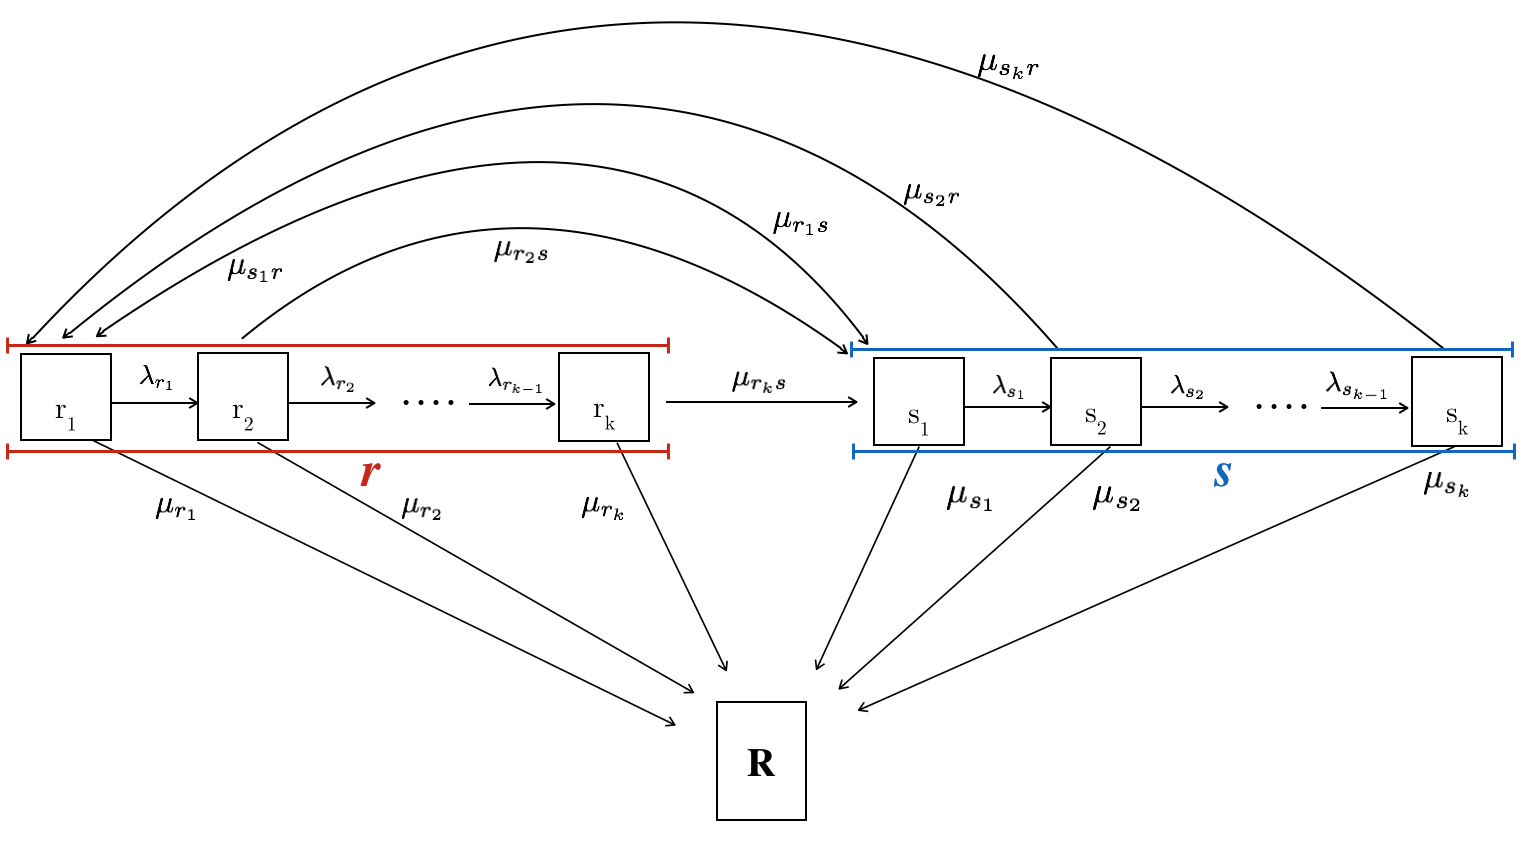
\includegraphics[scale=0.5]{coxmodelstitched2.png}
\caption{This figure summarizes the transition diagram of the underlying process $X^*(t)$. $r$, $s$ are any transient state of $X(t)$ with underlying $X^*(t)$ states $r_1,\ldots,r_k$ and $s_1,\ldots,s_k$ respectively, and $R$ is the only absorbing state.}
\end{figure}

Recall that $X(t)$ denotes a continuous time stochastic process with state space $\{1,\ldots, R\}$, where $t$ is time since process origin. Let $R$ be the only absorbing state. Underlying $X(t)$ there is the latent homogeneous CTMC $X^*(t)$ with latent state space $\{1_1,\ldots1_{s_1}\}\cup \ldots \cup \{(R-1)_1,\ldots (R-1)_{s_{R-1}} \cup R\} $. $X(t)=r \Leftrightarrow X^*(t) \in \{r_1,\ldots r_{s_r}\}$ for $r<R$ and $X(t)=R \Leftrightarrow X^*(t) =R$. The sojourn distribution of each non-absorbing state $r$ of $X(t)$ is assumed to be a $k$-phase Coxian phase-type distribution, defined to be the distribution of absorption time of a CTMC with $k$ progressive states and one absorbing state. Thus for observable state $r$, the latent process $X^* (t)$ can have the states $r_1,\ldots,r_k$,  with parameters $\lambda_{r_j}$ being the intensity for movement from $r_j$ to $r_{j+1}$, for $j=1,\ldots, k-1$, the assumption that the latent phases for each observable state is progressive makes all other transitions between $r_j$'s have $0$ intensity. $\mu_{r_j s}$ denotes the intensity for movement out of a latent phase of $r_j$ to state $s$. Coxian model has the assumption that any state $s$ is entered only at latent phase $s_1$, and so all other intensities for transition from latent phases of $r$ to latent phases of $s$ are $0$. Figure 1 summarizes the transition diagram of the underlying process $X^*(t)$. For greater estimability by reducing number of free parameters Titman \& Sharples (2010) assume that $\mu_{r_j s} = \tau_{r_j} \mu_{r_1 s} \forall s$, $\tau_{r_1}=1$. That is the rates of exiting from latent phase $r_j$ relative to $r_1$ change by the same factor irrespective of destination. 


\begin{figure}[t!]

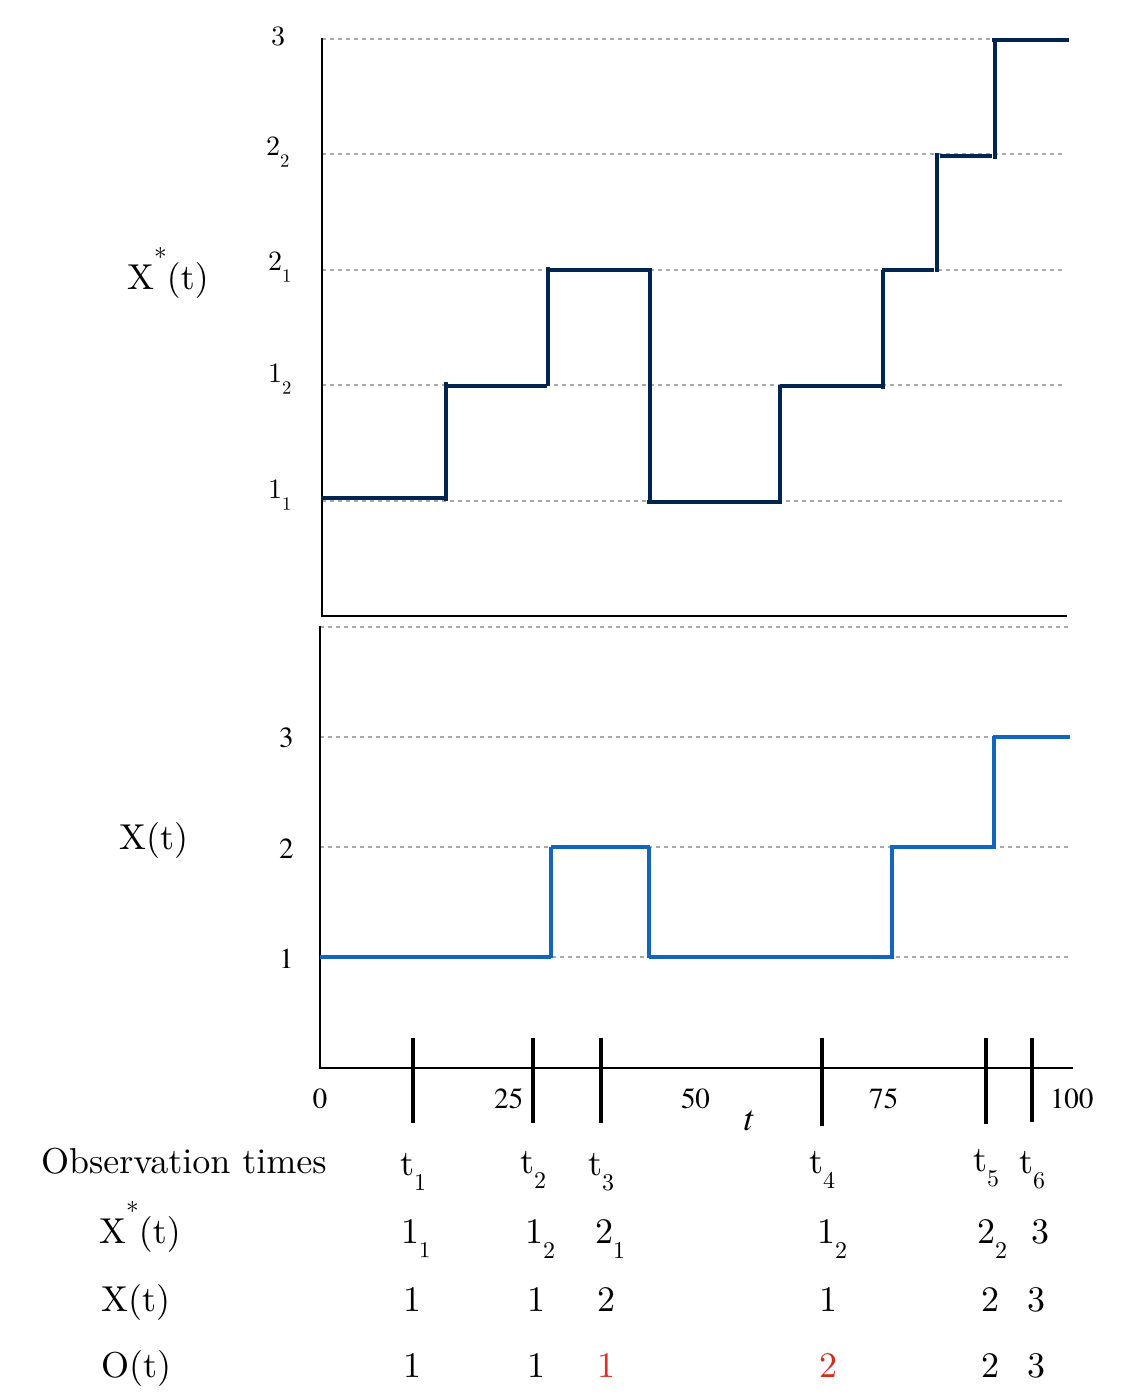
\includegraphics[scale=0.4]{figprocessAndsampling3.png}\hspace{10mm} 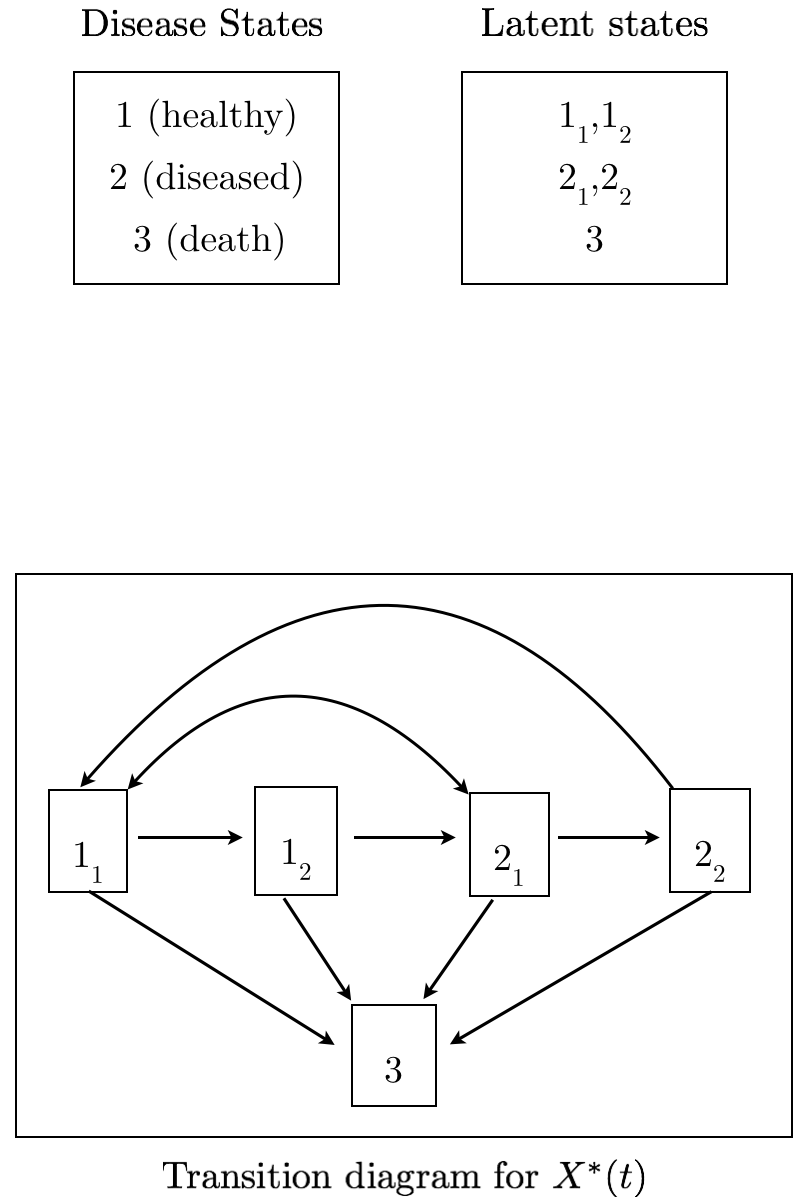
\includegraphics[scale=0.45]{datatransitions2.png}
\caption{Illustration of a disease process with latent trajectory $X^*(t)$, corresponding disease trajectory $X(t)$, and misclassified trajectory $O(t)$. The three states of the disease process $X(t)$ : \{1=healthy, 2= BOS, 3=death\} with $3$ the only absorbing state. $X(t)$ has underlying latent homogeneous CTMC $X^*(t)$ with state space $S^*=\{1_1,1_2,2_1,2_2,3\}$ where $\{3\}$ an absorbing state and the rest transient. $O(t)$ is the observed process which is the misclassified version of $X(t)$. States which are misclassified in this example are marked in red.}
\end{figure}

$X(t)$ is a semi-Markov process. To see this we view $X(t)$ as \[(\sigma_0,\tau_1,\sigma_1,\ldots.\tau_n,\sigma_n,\ldots),\]where the random variables $\sigma_0,\sigma_1,\ldots$ denote the initial and subsequent consecutive states occupied by the process, and let $\tau_n$ represent the sojourn time between the $(n - 1)$th and $n$th states, for $n \in \mathbb{N}$. Then the sequence of consecutively occupied states $\sigma_n$ forms a simple Markov chain, and the sojourn times between consecutively occupied states are independent random variables with distributions that depend only on the adjoining states, which implies that the process is semi-Markov (Cox and Miller, 1977). Note that the sojourn time in a state $\tau_n$ is a convolution of a random (yet, almost surely bounded) number of sojourn times in states of the latent process, which are exponentially distributed given states of latent process. Thus $\tau_n$ itself is in general not distributed exponentially given $\sigma_{n-1}$, that is $X(t)$ is not in general Markov.


To incorporate that the states in the process are observed with misclassification error, it is considered that observed states are $O(t)$ which are related to $X(t)$ by taking a value with misclassification probability $e_{rs}=P(O(t)=s|X(t) =r)=P(O(t)=s|X^* (t) =r_j) = e^*_{r_j s}$ for $r,s = 1,\ldots,R$, $j=1,\ldots, k$. The process $(O(t), X^*(t))$ is a Hidden Markov Model (HMM).  Thereby computational methods tailored for statistical analysis of HMMs can be used for inference. Since $X(t)$ is semi-Markov, the process $(O(t),X(t))$ is termed as a Hidden semi-Markov Model (HSMM). Figure 2 shows an example of a disease process with latent trajectory $X^*(t)$ and the corresponding disease trajectory $X(t)$ and misclassified trajectory $O(t)$ for a two-state reversible disease model.


\subsection{Inference and identifiability}

Denoting $o_0,\ldots, o_{n}$ to be the sampled observations with misclassification at times $t_0,\ldots,t_{n}$ for an individual, the latent HMM structure of the model enables to write the likelihood contribution for the individual based on the forward-backward algorithm (See Appendix A), as follows.

\begin{equation}\label{eqn:likelihood}
L=\pi \bm{M}_1^* \bm{M}_2^* \ldots \bm{M}_{n}^* \bm{1}
\end{equation}
where $\bm{M}_i^*$ is a $\{k(R-1) +1\} \times \{k(R-1) +1\}$ matrix with $(r^*,s^*)$ entry $e^*_{s^* o_i} p^*_{r^* s^*} (t_i - t_{i-1})$ for $r^*, s^* \in S^*$, with $\mathbf{P}^*(t)=\left\{p^*_{r^* s^*}(t)\right\} = e^{\bm{\Lambda}t}$,  and, $\pi$ is the initial state distribution.

The presence of misclassification and HMM setup increases possibility of non-identifiability (MacDonald \& Zucchini, 1997). In fact for a HMM with two states and balanced observation times, it is not possible to simultaneously identify the misclassification probabilities and transition intensities or probabilities without putting constraints, for instance that misclassification probabilities are each $<0.5$ (Rosychuk \& Thompson, 2003).

In addition, the Coxian phase-type structure induces non-identifiability. For example, the sojourn time distribution for state r is exponential if $\tau_{r_j} = 1 \forall j = 1,\ldots , k$. The parameters, $\lambda_{r_j}, j = 1,...,k - 1$, are redundant and unidentifiable in this situation.

As ensuring identifiability is not straightforward, the authors suggest inspection of the likelihood function by evaluating the Hessian matrix to ensure the estimated parameters are at a maxima and performing optimization procedures from a wide range of starting values to ensure a strict global maxima has been attained, or, checking for unimodality of the likelihood. If non-identifiability is evident, reduction of the complexity of the model can be attempted. Else, the parameters can be constrained. The authors suggest performing the optimization by first maximizing the profile likelihood on a grid of possible fixed values of the $\lambda_{r_j}$. Other possible constraints suggested are having some $\lambda_{r_j}$ as known constants, or constraining some of the sojourn distributions to be exponential.

Due to identifiability problems for exponential sojourn distributions in the current model, the likelihood ratio test for Markov versus Coxian phase-type semi-Markov model may not have an asymptotic $\chi^2$ distribution. Chen et. al (2001) proposed a penalized likelihood ratio tests for homogeneity in finite mixture models. Authors considered the same method but with an appropriate penalty for the current situation so that the $\lambda_{r_j}$'s are away from $0$ and $\infty$ and identifiable irrespective of value of $\tau$.

Titman \& Sharples (2008) proposed a goodness of fit test applicable for Markov and Hidden Markov Models. The same is used for testing gooness of fit in current model which  boils down to a HMM.
%Titman and Sharples (2010) discussed using a Coxian phase-type latent model whose observable process is semi-Markov. It has advantages in computation and  by an illness-death model with 3-states (of being well or in BOS or dead). It is assumed to be Semi-Markov. The data is panel observed at discrete time points with no information about the times or types of events between observations. Further, here the transition intensities are suspected to depend on the time since entry into a state, reason for not assuming homogeneity. The available data is considered to be realizations sampled at discrete time points (may be irregular) for each patient. It is assumed throughout, that, the sampling mechanism from the continuous process is non-informative (Gruger, Kay, Schumacher, 1991).

%$W(t)$ denotes the disease process with the three states : S = \{1=healthy, 2= BOS, 3=death\} with $3$ the only absorbing state. Titman and Sharples considered $W(t)$ to have an underlying latent homogeneous CTMC with state space $S^*=\{1_1,1_2,2_1,2_2,3\}$ with a 2-phase Coxian phase-type sojourn distribution with $\{3\}$ an absorbing state and rest transient, and rate matrix $\bm{\Lambda}$ constant with time.  If the latent process $X^*(t) \in {r_1,\ldots, r_k}$ then an accurately observed process $X(t) = r$, $r=1,2,~k=1,2$, if $X^*(t)=3$, $X(t)=3$. It is assumed that an individual enters transient state $r$ in phase $r_1$ and passes progressively through consecutive phases until the state is exited which can occur through any phase. Thus $\lambda_{r_j s_1}, r,s=1,2,~j=1,2, \lambda_{r_j,3}$ denote the underlying transition intensities of going from observable state $r$ to $s$. For greater estimability and practical interpretation of the intensities of moving out of a state to another, it is assumed that $\lambda_{1_1 2_2} = \tau_1 \lambda_{1_1 2_1}, \lambda_{1_2 3} = \tau_1 \lambda_{1_1 3}, \lambda_{2_2 1_1} = \tau_2 \lambda_{2_1 1_1}, \lambda_{2_2 3} = \tau_2 \lambda_{2_1 3} $. That is rates of exiting from state $1_2$ compared to $1_1$ change by the same factor irrespective of destination and similar for $2_2$ compared to $2_1$. In addition to these, transition intensities from phase $1_1$ to $1_{2}$ and from $2_1$ to $2_{2}$ are kept as parameters, and all other transition intensities of the latent process are 0. To incorporate misclassification, we consider $W(t)$ takes a value with misclassification probability $e_{rs}=P(W(t)=s|X(t) =r)=P(W(t)=s|X^* (t) =r_j)$ for $r,s =1,2, j=1,2$. It is noted that the process $(W(t), X^*(t))$ fits into the Hidden Markov Model framework (See also eqn. (1); so also called Hidden Semi Markov Model, HSMM). A better fitting model is recorded if the disease status is assumed unkown at the first observation time, and incorporating probability of initial states $\pi$ in the model, which is estimated from data.

%After a first analysis, $\pi_{1_2}$ and $\pi_{2_2}$ were estimated to be nearly $0$, so in the model a priori they were taken to be $0$, and $\pi_{1_1}=1-\pi_2$ (say), $\pi_{2_1}=\pi_2$.  Also, transplantation type was seen to have a significant effect on probability of initial state being 2, and on the probability of a state being misclassified as 2, given true state is 1. So they were  modelled as $logit(\pi_2) = a_0 + a_1 1(DL)$, and $logit(e_{12})=b_0 + b_1 1(DL)$, where $1(DL)$ is the indicator of double lung transplant.

%It is noted that the final quantities of interest, first passage cumulative distribution function, transition probabilities, hazard rates and survival probabilities are one-dimensional functionals of the parameter vector of the latent CTMC, and point and interval estimates of the former can be obtained from those of the later using Delta method.

\section{Application : Bronchiolitis obliterans syndrome}
Bronchiolitis obliterans syndrome (BOS) is the irreversible progressive narrowing of bronchiolar lumens and airflow obstruction (Todd \& Palmer, 2011), leading to impaired lung function. It is recorded to affect a majority of lung transplant recipients and is the principal factor limiting long-term transplant survival. It is measured by decline in forced expiratory volume in 1 second in liters $(FEV_1)$ relative to a posttransplanation baseline measure, with a level of 80\% of baseline or above deemed normal and less than 80\% is the clinical marker for BOS onset (Estenne et al, 2002). The primary scientific objectives are inferring on the rate of BOS onset, survival rate of patients before BOS onset, and, after BOS onset given survived for certain years after onset, and the extent of misclassification. The dataset includes 364 post-lung-transplant patients who received transplants at Papworth Hospital between 1984 and 2006, with 242 heart-lung transplant and 122 both-lung trasnplant patients. Patients were scheduled to for visit at 9 months, 12 months, after that at 6 month intervals, but actual visit times were highly irregular, and can be of different number, motivating modelling the process by on the time continuum.

\subsection{The methods applied to the BOS scenario}

\paragraph{The model} Titman and Sharples (2010) modelled the disease process on continuous time by an illness-death model with 3-states (of being well or in BOS or dead) (Fig 2). It is assumed to be a Semi-Markov process. The available data is considered to be realizations sampled at discrete time points (may be irregular) for each patient. It is assumed throughout, that, the sampling mechanism from the continuous process is non-informative (Gruger, Kay, Schumacher, 1991).

$O(t)$ denotes the disease process with the three states : S = \{1=healthy, 2= BOS, 3=death\} with $3$ the only absorbing state. Titman and Sharples considered $O(t)$ to have an underlying latent homogeneous CTMC as described in Section 2.3 with state space $S^*=\{1_1,1_2,2_1,2_2,3\}$ with $\{3\}$ an absorbing state and rest transient, and rate matrix $\bm{\Lambda}$ constant with time, and thereby a 2-phase Coxian phase-type sojourn distribution.  If the latent process $X^*(t) \in {r_1,\ldots, r_k}$ then an accurately observed process $X(t) = r$, $r=1,2,~k=1,2$, if $X^*(t)=3$, $X(t)=3$. We recall that an individual enters transient state $r$ in phase $r_1$ and passes progressively through consecutive phases until the state is exited which can occur through any phase. And $\mu_{1_2 2} = \tau_1 \mu_{1_1 2}, \mu_{1_2 3} = \tau_1 \mu_{1_1 3}, \mu_{2_2 1} = \tau_2 \mu_{2_1 1}, \mu_{2_2 3} = \tau_2 \mu_{2_1 3} $ (The notations for the transition intensities have been introduced in Section \ref{subsection : coxian}). In addition to these, transition intensities from phase $1_1$ to $1_{2}$ ($\lambda_1$) and from $2_1$ to $2_{2}$ ($\lambda_2$) are kept as parameters, and all other transition intensities of the latent process are 0. To incorporate misclassification, we consider $O(t)$ takes a value with misclassification probability $e_{rs}=P(O(t)=s|X(t) =r)=P(O(t)=s|X^* (t) =r_j)$ for $r,s =1,2, j=1,2$. $(O(t), X^*(t))$ is a Hidden Markov Model (See also eqn. (1); so also called Hidden Semi Markov Model, HSMM). A better fitting model is recorded if the disease status is assumed unknown at the first observation time, and incorporating probability of initial states $\pi$ in the model, which is estimated from data.

After a first analysis, $\pi_{1_2}$ and $\pi_{2_2}$ were estimated to be nearly $0$, so in the model a priori they were taken to be $0$, and $\pi_{1_1}=1-\pi_2$ (say), $\pi_{2_1}=\pi_2$.  Also, transplantation type was seen to have a significant effect on probability of initial state being 2, and on the probability of a state being misclassified as 2, given true state is 1. So they were  modelled as $logit(\pi_2) = a_0 + a_1 1(DL)$, and $logit(e_{12})=b_0 + b_1 1(DL)$, where $1(DL)$ is the indicator of double lung transplant.

It is noted that the final quantities of interest, first passage cumulative distribution function, transition probabilities, hazard rates and survival probabilities are one-dimensional functionals of the parameter vector of the latent CTMC, and point and interval estimates of the former can be obtained from those of the later using Delta method (See Appendix B).

\paragraph{Parameter estimation and Computation}
The authors kept only the nearest observation to a scheduled visit time and excluded others from analysis, for each patient, as an attempt to ensure non-informative sampling. The likelihood contribution for the individual based on the forward-backward algorithm is recorded in Equation \ref{eqn:likelihood} where now each $\bm{M}_i^*$ is a $5\times 5$ matrix and $\pi=(1-\pi_{2},0,\pi_{2},0,0)$ is taken as the initial probabilities.

The 13 parameters are estimated by a maximum likelihood estimate (MLE) considering all patients. To check for global optimum, we computed the MLE from 30 random starting values. Full optimization was then performed starting at the best value among the 30 MLEs. We used the quasi-Newton algorithm due to Broyden, Fletcher, Goldfarb and Shanno (BFGS, 1970) to maximize likelihood and obtain point and interval estimates of the model parameters, with a default relative convergence tolerance of 'optim' ($10^{-8}$) and capped likelihood evaluations at $2500$.

Hypothesis tests of significance of different parameters were performed  by using the penalised likelihood ratio test (Chen et al., 2001) to account for non-identifiability in the current setup. It has an approximate $\chi^2$ distribution. Since the setup becomes that of a HMM, the authors used a Pearson-type goodness of fit test for HMMs proposed by them (2008) to assess the overall fit of the data.
\section{Results}
The model parameter estimates are similar, but not identical to those obtained by Titman and Sharples (2010), because of differences between the two datasets. Table 1 shows MLEs and 95\% confidence intervals for the parameters of the model. The MLEs were unique on the basis of numerical investigations with different starting values. In both the HMM and HSMM, $\mu_{1_1 3}<\mu_{2_1 3}$ showing that as expected the transition rate to death is estimated to be higher for patients with BOS than those without. The BIC depicts a better fit for the HSMM model.


The first passage CDF for BOS development is reported in Fig 3a. The probability of an individual remaining BOS free at 5 years post transplant given initially healthy is 28\%, with a 95\% confidence interval of (22\%, 38\%). This is in agreement with existing literature where existing estimates of a 5 year disease free probability were between 15\% and 37\% (Chan, Allen; 2004). The model predicts that the rate of entry into the diseased states decrease with time since transplant; Initially disease rates are 35\%–40\%, and decrease to 18\% per year after 5 years (Figure 3b). Heterogeneity in the lung transplant patient population in terms of progression to BOS might have led to the nonconstant disease hazard of BOS. Decreasing BOS rates are agreeing with the fact that risk for experiencing infections or acute rejection episodes, which may trigger BOS development, is high at the initial period right after transplant (Jackson et al., 2002).

\begin{table}
\centering



\resizebox{6in}{!}{%
\begin{tabular}{ccccccc}
\hline
Intensiy rates & \thead{Transition\\ i} & \thead{\\j} & HMM point estimate & HMM 95\% CI & HSMM point estimate & HSMM 95\% CI\\
\hline
& $1_1$ & $1_2$ & & & 0.40 & (0.11,0.48) \\
& $1_1$ & $2_1$ & 0.12  & (0.09,0.15) & 0.38 & (0.27,0.55)\\
& $1_1$ & $3$ & 0.04 & (0.03,0.07) & 0.01 & (0.00,0.026)\\
& $1_2$ & $2_1$ & & & 0.17 & (0.12,0.25)\\
& $1_2$ & $3$ & & & 0.01 & (0.00,0.12 )\\
& $2_1$ & $2_2$ & & & 7.97 & (0.19,36.03)\\
& $2_1$ & $1_1$ & 0.03 & (0.01,0.13) & 1.00 & (0.18,5.72)\\
& $2_1$ & $3$ & 0.25 & (0.20,0.30) & 2.41 & (0.11,5.76)\\
& $2_2$ & $1_1$ &  &  & 0.04 & (0.02,0.08)\\
& $2_2$ & $3$ &  &  & 0.21 & (0.16,0.28)\\
\hline
\hline
Emission & e(Healthy, BOS) & Heart Lung & 0.50 & (0.50,0.50) & 0.507 & (0.506,0.507)\\
& & Double Lung & 0.50 & (0.50,0.50) & 0.77 & (0.71,0.83)\\
& e(BOS, Healthy)& & 0.526 & (0.524,0.527) & 0.50 & (0.5019,0.5021)\\
\hline
\hline
Initial distribution & $\pi(\mbox{BOS}_1)$ & Heart Lung & 0.50 & (0.50,0.50) & 0.523 & (0.522,0.530)\\
& & Double Lung & 0.50 & (0.50,0.50) & 0.70 & (0.64,0.78)\\
\hline
\hline
- Log-likelihood & & & \multicolumn{2}{c}{-2533.91} & \multicolumn{2}{c}{-1619.88}\\
BIC & & & \multicolumn{2}{c}{5120.89} & \multicolumn{2}{c}{3316.41}\\
No. pars & & & \multicolumn{2}{c}{9} & \multicolumn{2}{c}{13}\\
\hline
\end{tabular}
}
\vspace{2mm}
\caption{Maximum likelihood estimation for model intensity rates, emission probabilities, and initial probabilities based on hidden Markov and phase-type HSMMs.}

\end{table}

\begin{figure}[]
\centering
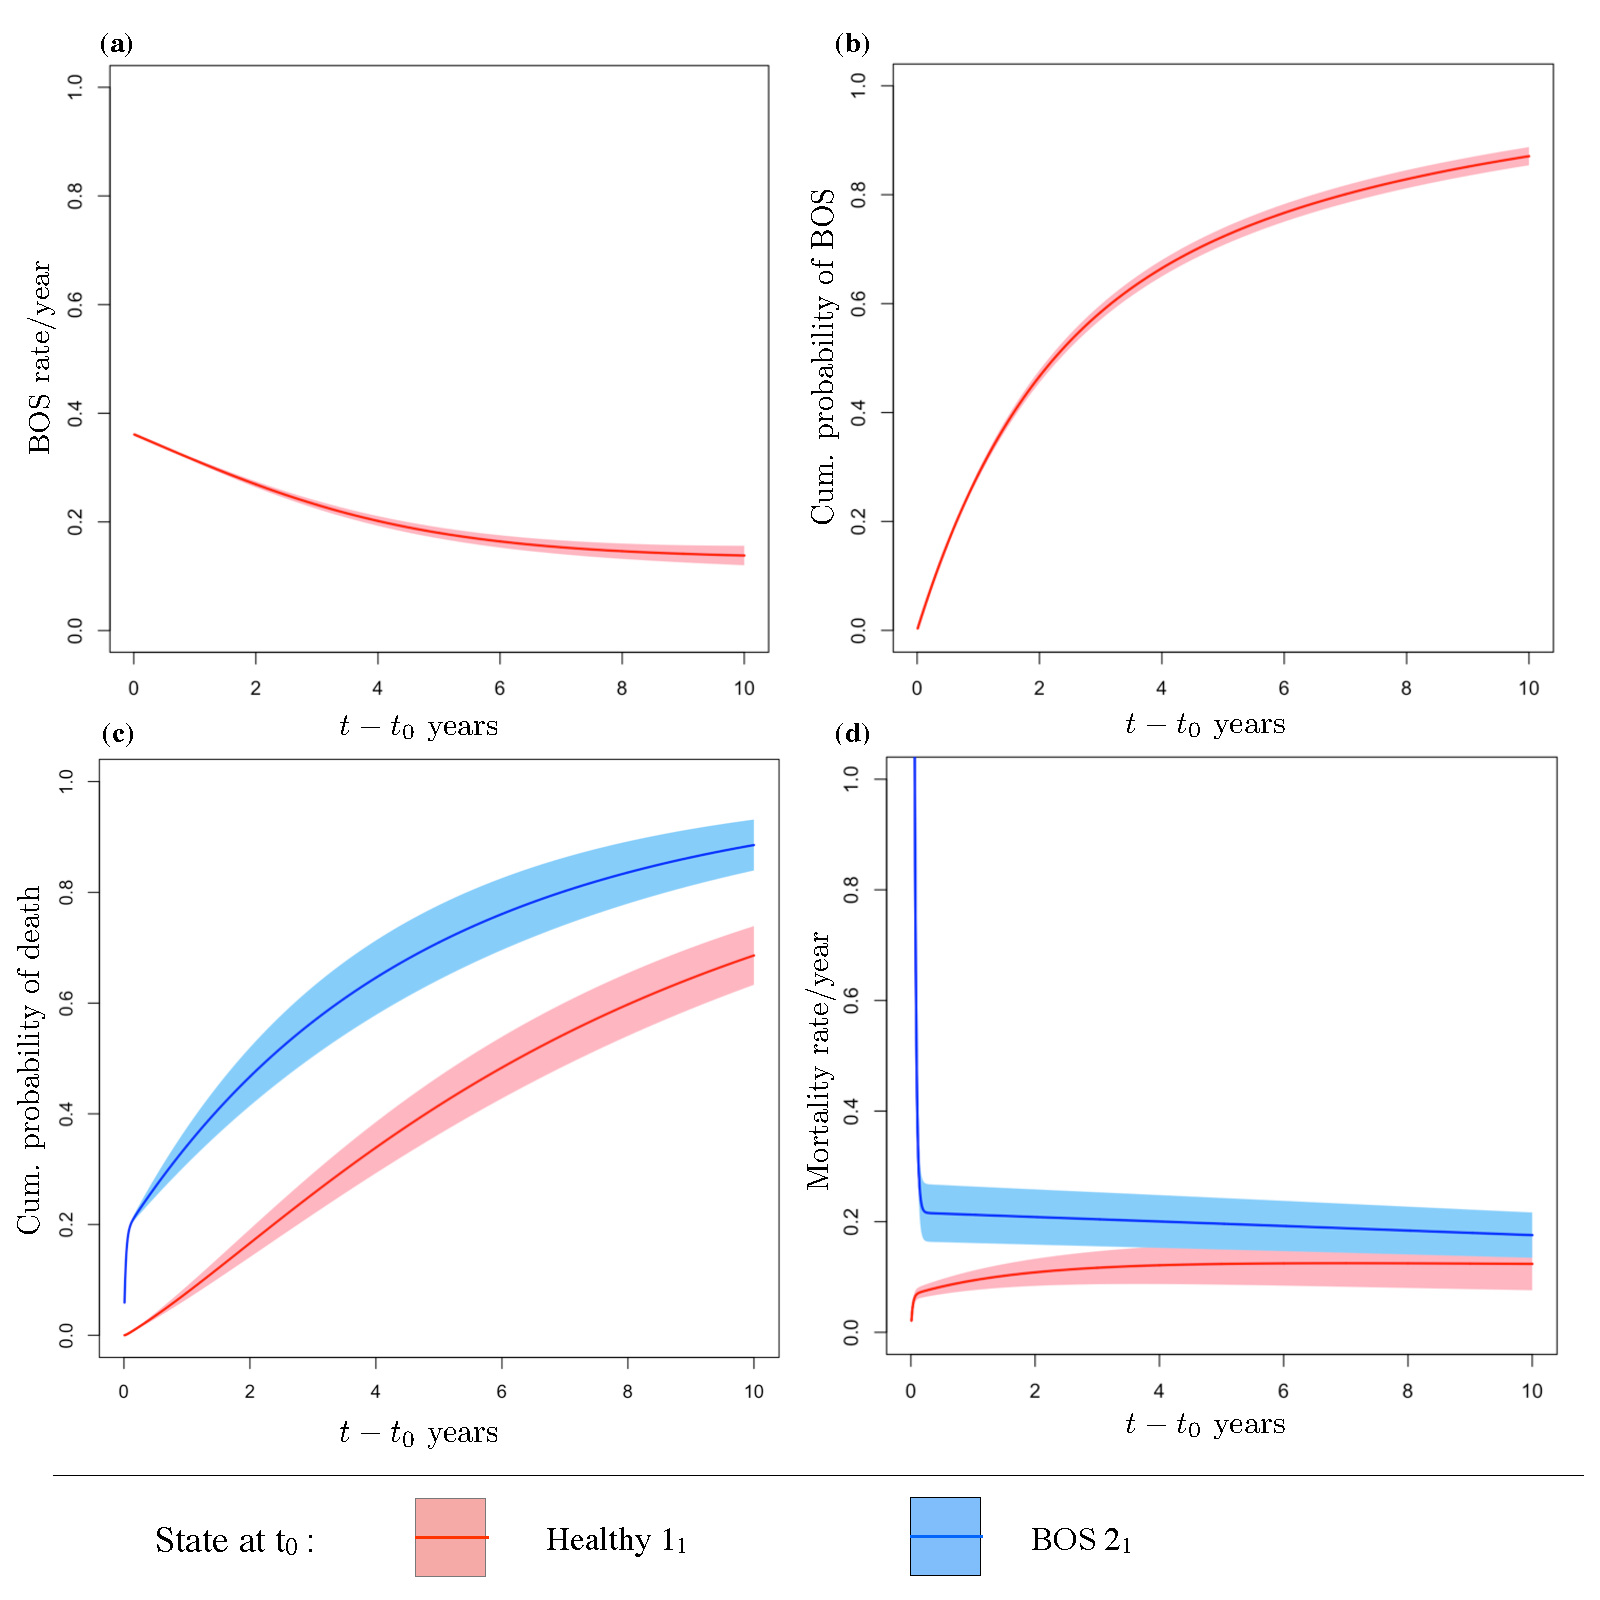
\includegraphics[scale=0.45]{4plots4.pdf}
\caption{(a). Disease rate conditional on being in healthy state $1_1$ at $t_0$. (b). Cumulative probability of having transitioned to BOS state at least once, conditional on being in $1_1$ at $t_0$. (c). Cumulative probability of death. (d). Mortality rate per year, as a function of state at $t_0$. In all figures, the shaded regions represent 95\% point-wise confidence intervals for the estimates.
}
\end{figure}


\begin{figure}
\centering
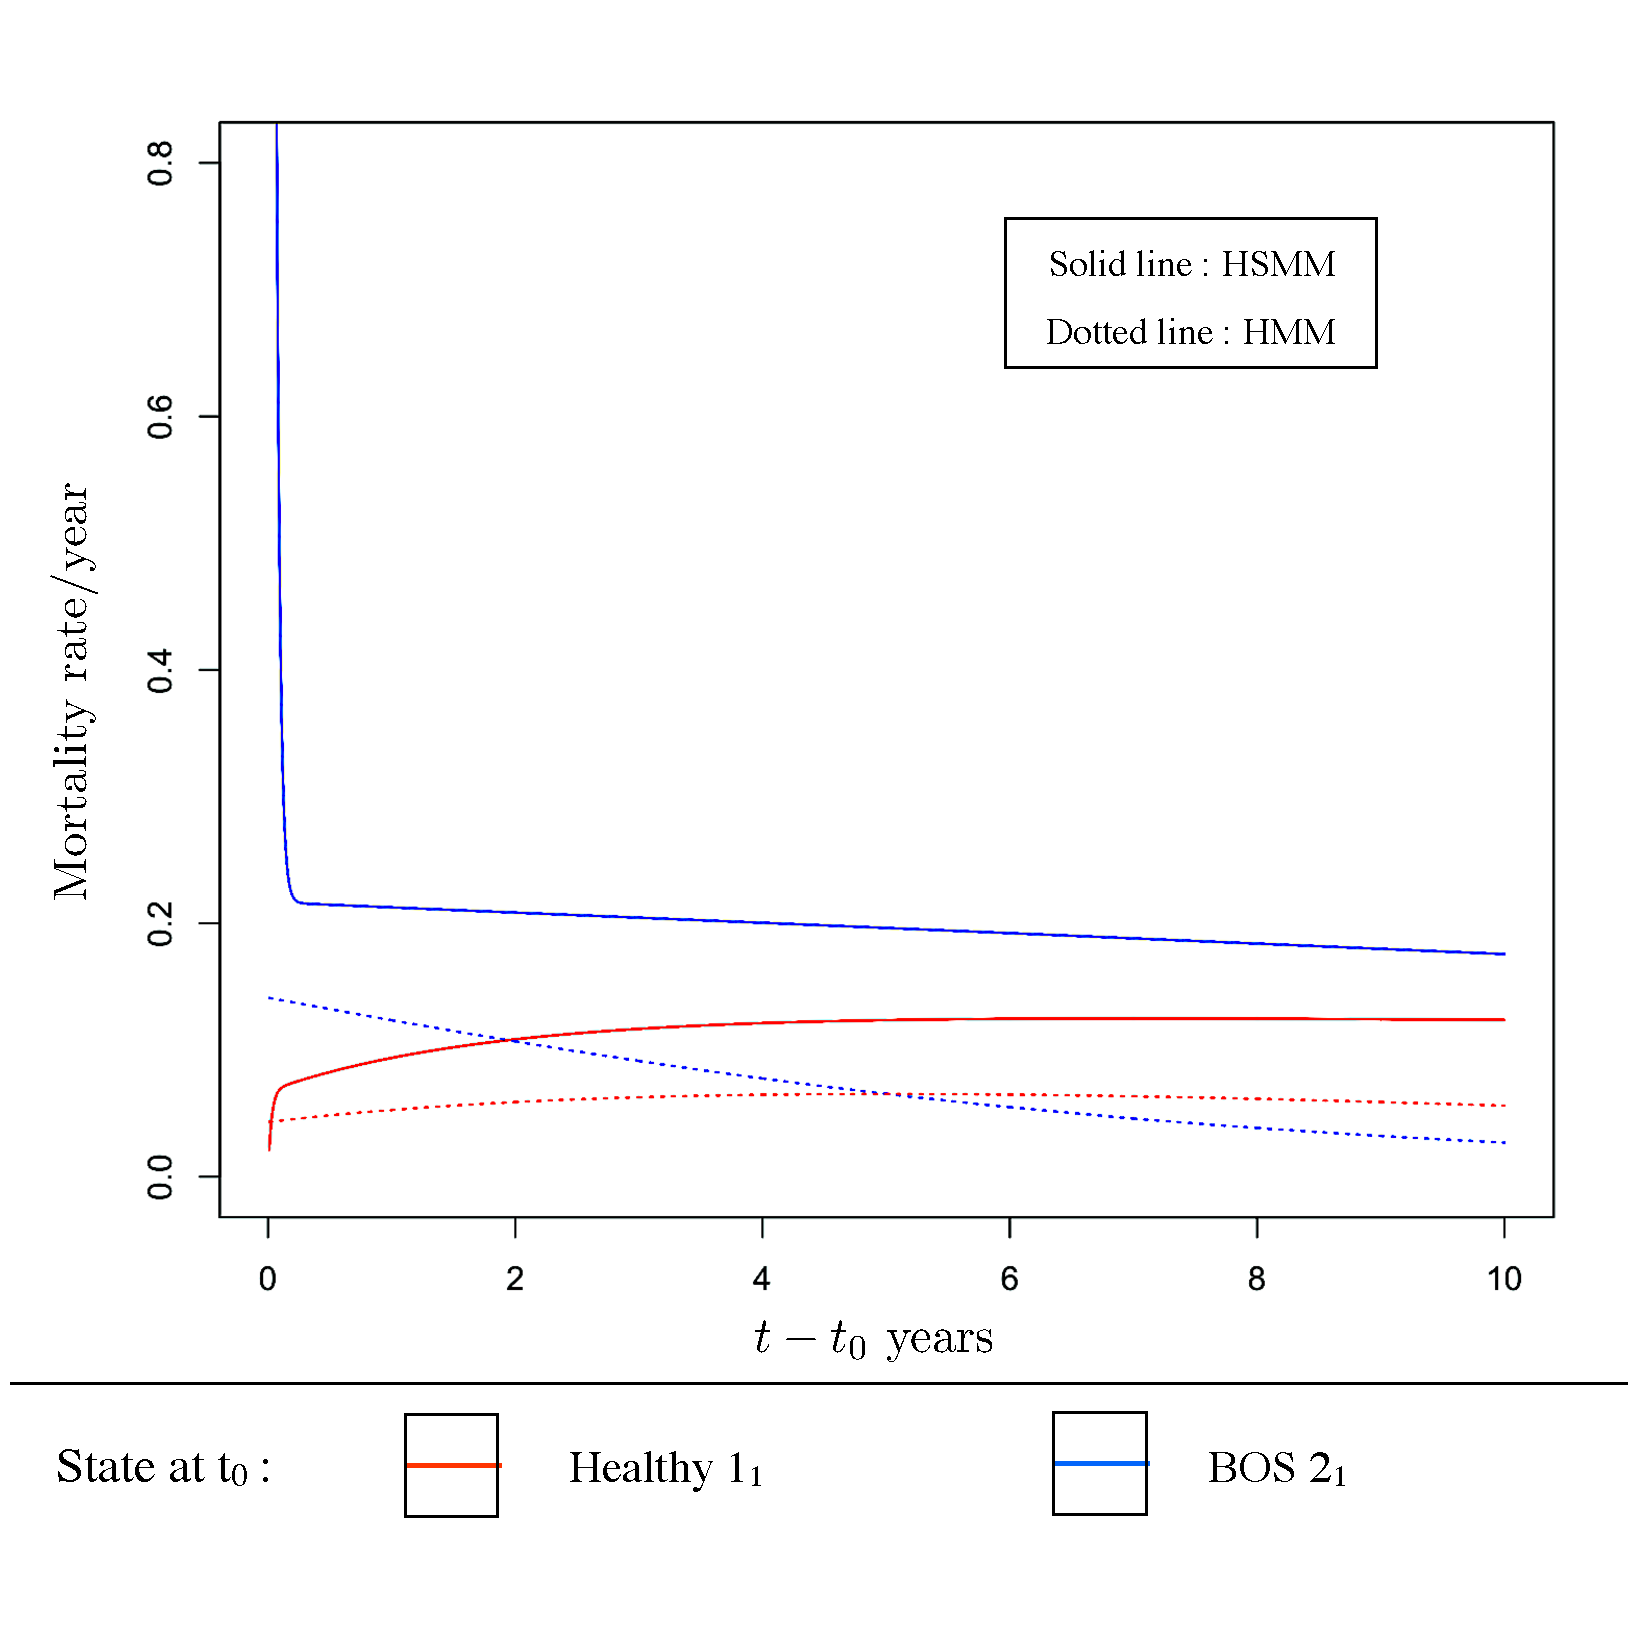
\includegraphics[scale=0.33]{mortcomp_hsmmhmmkey.pdf}
\caption{Mortality rate per year, as a function of state at $t_0$ for the HSMM and HMM models.}
\end{figure}

The cumulative probabilities of death given initial state is healthy versus BOS are plotted in Fig 3c. By 2 years post transplant, about 17\% of those healthy at the beginning of the study are estimated to have died. After BOS initiation, about 66\% remain alive for 1 year, 43\% for 3 years, 29\% for 5 years. These estimates are in agreement with the literature estimates of survival after bilateral lung transplant of 74\%, 46\%, and 26\% at 1, 3, and 5 years after the onset of BOS, respectively (Finlen et al., 2010).

In Fig. 3d, we note that till before BOS onset, mortality rates are very low. After having BOS onset, mortality rates increase drastically to $>50\%$ per year, and then decrease to 20\% after 2 years, followed by a gradual decline in rate. This trend is reminiscent of the identification of distinct BOS patient populations: those with acute onset and rapidly deteriorating lung function, and those with more gradual onset and slowly progressing disease (Jackson et. al, 2002; Lama et. al, 2007).


In Fig. 4 we note that unlike the HSMM model, the HMM model did not show the detailed artifacts of the disease mortality rates which is backed by the medical literature.

We computed the MLE by the HSMM model over 30 random starting values from independent Normal (mean=0,sd=0.25) (See Fig. 5). The median run-time of the HSMM optimization over 30 runs was 4395.43 seconds. Presence of multiple local maxima where the algorithm converged (Fig. 5), and, non-identifiability that is, different parameters (Table 2) leading to approximately same likelihood with same integer parts has been recorded in the process.



A Pearson-type goodness of fit test (Titman \& Sharples; 2008, See Appendix D) for the HSMM  model stratified by transplant type (heart lung or double lung), observation number in an individual’s series ($\leq 6$ or $>6$), time elapsed since last observation (for observation number $\leq 6$, time elapsed categories : $\leq 0.44$ years, $> 0.44$ years. for observation number $> 6$ and time elapsed categories : $\leq 0.51$ years, $> 0.51$ years). The statistic had a value of 36.92. The null distribution of the statistic cannot be accurately calculated without bootstrapping, which would be time consuming for the current algorithm. However $\chi^2(D) (0.95)$ is an upper bound to the $95\%$ quantile of the statistic (Titman \& Sharples; 2008), where $D$ denotes the number of independent cells. In this case $D = 32$ which gives the upper bound as 46.2. Thus this test does not provide strong evidence in favor of poor fit. The goodness of fit test in the HMM setup gives evidence for a poor fit with test statistic of 96.81 on $\chi^2_{24}$ distribution.


\begin{table}
\centering
\resizebox{5.5 in}{!}{%
\begin{tabular}{cccccccccccccc}
\hline
$\lambda_1$ & $\mu_{1_1 2}$ & $\mu_{1_1 3}$ & $\tau_{1_2}$ & $\lambda_2$ & $\mu_{2_1 1}$ & $\mu_{2_1 3}$ & $\tau_{2_2}$ & $e_{21}$ & $e_{12}^{HL}$ & $e_{12}^{DL}$ & $\pi_{HL}$ & $\pi_{DL}$ & $-LL$\\
\hline
0.12 &  0.34 &  0.00 & 0.27 & 36.25 &  1.24 &  8.51 &  0.03 &  0.01 &  0.51 &  0.80 & 0.53 & 0.56 & 1615.143\\
0.26 & 0.35 & 0.03  & 0.37 & 5.11 & 0.18 & 1.31 & 0.16 & 0.01 & 0.51 & 0.79 & 0.52 & 0.77 & 1615.261\\
\hline
\end{tabular}
}
\vspace{2mm}
\caption{This is a demonstration of non-identifiability of the likelihood for the BOS dataset. Two different parameter sets lead to approximately the same likelihood.}
\end{table}
\begin{figure}
\centering
\includegraphics[scale=0.6]{ll_timetaken.pdf}
\caption{Runtime and attained LL using BFGS algorithm to fit the BOS data, using 30 random starting values}
\end{figure}


We performed an hypothesis test with null hypothesis of HMM versus an alternative of HSMM by a modified likelihood ratio test based on Chen et al., 2001 (Appendix C). The value of the test statistic was 25.18. The test statistic has an approximate $\chi^2(2)$ distribution whose $95\%$ quantile is nearly $5.99$. Therefore, this shows strong evidence against the HMM model in favor of the HSMM model.

Although, biologically, BOS is an irreversible disease, Titman and Sharples (2010) decided to include a BOS $\rightarrow$ healthy transition in their latent CTMC model. Titman \& Sharples recorded a likelihood ratio test in the standard CTMC HMM setup, whence there was support that including a BOS $\rightarrow$ healthy transition leads to significant improvement in fit. As an additional test, not reported by Titman and Sharples (2010), we decide whether to include BOS $\rightarrow$ healthy transition in the HSMM setup. That is we compare the null hypothesis of HSMM model without the BOS $\rightarrow$ healthy transition versus the alternative of an HSMM model with this transition. The test statistic is 9.038. The null hypothesis (the transition between BOS to healthy states has a rate of zero) is on the boundary of the parameter space; thus the distribution of the likelihood ratio test statistic is not a standard chi-square distribution, but rather a 50:50 mixture of a chi-square with 1 df and a point mass at zero (Self and Liang, 1987). The p-value for the LR test statistic was 0.0013, which supports the hypothesis that the reversible transition improves the fit within the latent disease framework.

\section{Discussion}

In modelling panel observed finite state processes, the widely-used approach of assuming standard CTMCs leads to models that are unrealistic for processes with duration-dependent sojourn distributions. Assuming a latent CTMC framework with misclassification accommodates duration-dependent sojourn distributions but yields tractable likelihoods levereging its Hidden Markov Model property. These models are also scientifically interpretable, as functionals describing the process are computable analytically.

On the BOS dataset, the results from the HSMM model consisted of detailed artifacts of the disease process matching with the medical literature, unlike the HMM method. BIC, and Pearson-type goodness of fit test depicted strong evidence that HMM model has a low fit, but not so for the considered HSMM model. Test for HMM vs HSMM based on Chen et al (2001) also resulted in strong evidence in favor of HSMM. We also recorded evidence that in the latent model setup keeping the BOS $\rightarrow$ healthy transition improves fit of the model.

The convergence of the BFGS algorithm for the data was slow, with a median runtime of 4395.43 seconds. The maxima also depended upon starting values. It is also seen that not much effort is made in the Titman \& Sharples (2010) paper to obtain a global maximum of the likelihood surface. To embetter on this Lange \& Minin (2013) proposed an EM algorithm for this setup, which is efficient and robust and outperformed optimization methods, like Nelder-Mead and BFGS, for a slightly different BOS dataset.

An advantage of latent CTMC models is their ability to approximate important functionals of disease processes like hazard functions from non-exponential sojourn time distributions. However, the authors record a general problem in panel observed setting. Due to the lack of information in the data, the transition intensities at times soon after entry into a state may be difficult to estimate because of the absence of consecutive observations in short time intervals leading to boundary maximum likelihood estimates. Similarly, when there is little evidence against a Markov model in the data optimization algorithms such as Nelder-Mead or Baum-Welch may fail to find the global maximum.

A further extension to the model could be to allow time dependence with respect to calendar time. Existing approaches to fitting time inhomogeneous Markov models based on parametric assumptions such as piecewise constant intensities can, in principle, be applied to the underlying latent Markov process. However, as with other possible model extensions, incorporating time inhomogeneity will increase the possibility of nonidentifiability.

In future the feasibility of obtaining robust variance estimates can be studied, although an implementation in this panel data context may require substantial improvement in speed of computation (Elashoff and Ryan, 2004).

In the presence of non-identifiable parameters, penalized likelihood ratio tests allow for hypothesis testing of the latent CTMC semi-Markov model against a CTMC model (Chen et al., 2001). Currently, for the latent CTMC context this test is limited to null models with exponential sojourn distributions (Titman and Sharples, 2010). By using an efficient fitting algorithm (Lange \& Minin ;2013) it can be possible to test more general models by k-fold cross validation with prediction error measured by a goodness of fit statistic (Titman and Sharples, 2008).

The present paper has focused on frequentist estimation. Bayesian methods have also fared well in current scenario (Bladt et al., 2003). Sensible priors may yield identifiable latent parameters, and posterior distributions provide uncertainty estimates for model functionals. McGrory et al. (2009) have discussed a full Bayesian approach to inference for Coxian phase type model with unknown number of phases and covariate dependent mean. Estimation of parameters including number of phases (that is model selection) is done by an implementation of reversible jump Markov Chain Monte Carlo (Green, 1995). They applied the method to a dataset on length of hospital stay.

Further, violation of the assumption of non-informative sampling is doubted by the authors in Titman \& Sharples (2010) to have occured and having adverse impact on modelling, but no rigorous check for that had been done and steps taken. Similar is the case for violation of independent misclassification assumption conditional on underlying chain. As one possible mitigation, Lange et al. (2015) proposed incorporating random disease driven observation times in the current latent CTMC setup, by keeping them as a Poisson process with rates depending on the patient's present disease status. It discusses model selection by BIC and estimation by EM algorithm similar to Item 1. Here also, Bayesian approaches as discussed in previous paragraph could come to use in addressing non-identifiability and model selection.

\bibliography{report}
\bibliographystyle{apalike}

\section*{Appendix}
\subsection*{A : Likelihood for HMM by forward-backward algorithm}\label{Appendix : A}
Let $S$ to be the finite state space of continuous time HMM $(O(t),X^*(t))$ with intensity matrix $\Lambda$ and emission probabilities $e_{i o}=P(O(t)=o|X^*(t)=i)$. Denoting $o_0,\ldots, o_n$ be the observations at times $t_0,\ldots,t_n$, let us define
\[
\alpha_n(i) = \mathbf{P}(O_{t_0}=o_o,\ldots, O_{t_n}=o_n,X^*_{t_n}=i)
\]
\[
\alpha_0(i)=\pi_i e_{i~ o_0}
\]

Now for $0\leq m\leq n-1, j\in S$,
\begin{align*}
\alpha_{m+1}(j)&=\mathbf{P}(O_{t_0}=o_o,\ldots, O_{t_{m+1}}=o_{m+1},X^*_{t_{m+1}}=i)\\
&=\sum_{i=1}^{|S|} \mathbf{P}(O_{t_0}=o_0,\ldots,O_{t_{m+1}}=o_{m+1},X_{t_m}=i,X_{t_{m+1}}=j)\\
&=\sum_{i=1}^{|S|}\mathbf{P} (O_{t_{m+1}}=o_{m+1}|X_{t_{m+1}}|=j) \mathbf{P}(X_{t_{m+1}}=j|X_{t_m}=i)\\
& \qquad \mathbf{P}(O_{t_0}=o_0,\ldots,O_{t_{m+1}}=o_{m+1},X_{t_m}=i)\\
&\mbox{ (Markov property of } X(t) \mbox{, and emission-transition diagram of HMM})\\
&=\sum_{i=1}^{|S|} e_{j o_{m+1}} p_{ij}(t_{m+1}-t_m) \alpha_m(i)\\
&=\left[\sum_{i=1}^{|S|}\alpha_m(i)p_{ij}(t_{m+1}-t_m)\right]e_{j o_{m+1}}\\
&=\left(\alpha_m(1),\ldots,\alpha_m(|S|)\right) \left(\begin{matrix}
p_{1j}(t_{m+1}-t_m)\\
p_{2j}(t_{m+1}-t_m)\\
\vdots\\
p_{|S|j}(t_{m+1}-t_m)
\end{matrix}\right) e_{j o_{m+1}}
\end{align*}
Therefore,
\begin{align*}
\left(\alpha_{m+1}(1),\ldots,\alpha_{m+1}(|S|)\right)=\left(\alpha_{m}(1),\ldots,\alpha_{m}(|S|)\right) \left(\left(p_{ij}(t_{m+1}-t_m)\right)\right)=\left(\alpha_{m}(1),\ldots,\alpha_{m}(|S|)\right) M_{m+1},
\end{align*}
denoting $M_{m+1}= \left(\left(p_{ij}(t_{m+1}-t_m)e_{j o_{m+1}} \right)\right) $.

Therefore,
\[
\left(\alpha_{n}(1),\ldots,\alpha_{n}(|S|)\right)=\left(\alpha_{0}(1),\ldots,\alpha_{0}(|S|)\right)M_1\ldots M_n = \left(\pi_1^*,\ldots,\pi_{|S|}^*\right) M_1\ldots M_n
\]
denoting constants $\pi_j^*=\alpha_{0}(j)$.
Therefore, since we have likelihood $L=P(O_{t_0}=o_0,\ldots,O_{t_n}=o_n)=\sum_{i=1}^n\alpha_n = \left(\alpha_1,\ldots,\alpha_n\right)\mathbf{1}$, we thus have
\[
L=\left(\pi_1^*,\ldots,\pi_{|S|}^*\right) M_1\ldots M_n \mathbf{1} = \pi M_1\ldots M_n \mathbf{1},
\] where $\pi=\left(\pi_1^*,\ldots,\pi_{|S|}^*\right)$.
\subsection*{B : Delta method standard errors of disease process functionals}
Suppose $\psi$ is a $p\times 1$ vector of latent model parameters with MLE $\hat{\psi}$, and $F(\psi, t)$ is a one-dimensional functional. Let $\nabla F (\hat{ψ}, t)$ be the $p \times 1$ gradient of $F (\psi, t)$ with respect to $\psi$ evaluated at $\hat{\psi}$. By the functional delta method, the asymptotic distribution of the functional estimates $F(\hat{\psi},t)$ is normal with mean $F(\psi,t)$ and an approximate covariance matrix given by
\[
Cov(F(\hat{\psi},t))=\nabla F(\hat{\psi},t)T Cov(\hat{\psi},t)\nabla F(\hat{\psi},t).
\]

Functionals such as CDFs, hazard functions, and transition probabilities are related to transition intensity by the matrix exponential. Thus the expression of derivative of $\exp(\Lambda(\psi)t)$ with respect to entries of $\psi$ would be useful for this. These derivative involve similar integrals as first moments of occupancy durations and transition counts and are computed with similar methods (Najfeld, Havel; 1994). For example, consider the functional $P_{ij}(t,\psi) = \exp (\Lambda(\psi)t)_{ij}$. Then $\frac{\partial P_ij(t,psi)}{\partial \psi [k]}$ is the $i,j$th entry of the matrix given by \[\int_{0}^t \exp (\Lambda (\psi) \tau) B_{\psi [k]} \exp (\Lambda (\psi) (t-\tau)) d \tau\] 
where $B_{\psi [k]} = \frac{\partial \lambda_{ij} (\psi)}{\partial \psi [k]}$. Next we consider the hazard function $h_{ij}(t,\psi)$ to absorbing state $j$  at time $t$ when initially at state $i$. \begin{align*}
\frac{\partial h_{ij}(t,psi)}{\partial \psi [k]} &= \frac{\partial}{\partial \psi [k]} \frac{\frac{\partial}{\partial t}P_{ij}(t,\psi)}{1-P_{ij}(t,\psi)}\\
& =\frac{(1-P_{ij}(t,\psi))\frac{\partial}{\partial \psi [k]} \frac{\partial}{\partial t}P_{ij}(t,\psi)- \frac{\partial}{\partial t}P_{ij}(t,\psi)\frac{\partial}{\partial \psi [k]} (1-P_{ij}(t,\psi))}{(1-P_{ij}(t,\psi))^2}\\
& =\frac{(1-P_{ij}(t,\psi)) \frac{\partial}{\partial t}\frac{\partial}{\partial \psi [k]}P_{ij}(t,\psi) + \frac{\partial}{\partial t}P_{ij}(t,\psi)\frac{\partial}{\partial \psi [k]} P_{ij}(t,\psi)}{(1-P_{ij}(t,\psi))^2}\\
&= \frac{(1-e^{\Lambda (\psi) t}_{ij}) e^{\Lambda (\psi) t} B_{\psi [k]} + (e^{\Lambda (\psi) t} \Lambda (\psi) )_{ij} e^{\Lambda (\psi) t} B_{\psi [k]}}{(1-e^{\Lambda (\psi) t}_{ij})^2}
\end{align*}
using the expression for $\frac{\partial P_ij(t,psi)}{\partial \psi [k]}$ above, and noting that $P(t)= \exp(\Lambda t)$ and $\frac{\partial}{\partial t} P(t) = \exp(\Lambda t) \Lambda$.
\subsection*{C : Modified LRT based on Chen, Chen, Kalbfleisch (2001)}
The following penalised likelihood $pl(\theta)$ is maximized
\[
pl(\theta) = l(\theta) + \sum_{j}\sum_{r} (C_{r_j} \log \lambda_{r_j} - C_{r_j} \lambda_{r_j} \alpha_{r_j})
\]
\subsection*{D : Goodness of fit test for HMM, Titman \& Sharples (2008)}

\end{document}